\documentclass[a4paper,12pt]{report}
\usepackage[utf8]{inputenc} % Kodierung
\usepackage[ngerman]{babel} % Sprache
\usepackage{geometry} % to change the page dimensions
\geometry{left=2.5cm, right=2cm, top=3cm, bottom=3cm} % or letterpaper (US) or a5paper or....
% \geometry{margin=2in} % for example, change the margins to 2 inches all round
% \geometry{landscape} % set up the page for landscape
%   read geometry.pdf for detailed page layout information
\usepackage{graphicx}
\usepackage{float}
\usepackage{fancyhdr}
\usepackage[bottom,hang]{footmisc}
\usepackage{tabularx}
\usepackage{setspace} % Paket für Zeilenabstand
\usepackage{acronym} % Paket für Abkürzungsverzeichnis
\usepackage[numbers,square]{natbib} % numbers ist notwendig für alphadin, squar sorgt für eckige Klammern
\usepackage{url}

%\setlength{\textwidth}{14cm}
%\setlength{\textheight}{25.5cm}
%\setlength{\topmargin}{-2.0cm}
%\setlength{\oddsidemargin}{0cm}
%\setlength{\evensidemargin}{0cm}

\fancypagestyle{plain}{
\fancyhead{}
\renewcommand{\headrulewidth}{0.0pt}}

\pagestyle{fancy}
\renewcommand{\chaptermark}[1]{\markboth{#1}{}}
\fancyhf{}
\fancyhead[R]{}
\fancyhead[L]{\textbf{\nouppercase\leftmark}}
\fancyfoot[R]{\thepage}
\fancyfoot[L]{}
\renewcommand{\headrulewidth}{0.5pt}

% 1.5 facher Zeilenabstand
\onehalfspacing
% weniger Silbentrennung aber dafür mehr Wortzwischenräume
\sloppy

\begin{document}

%===================================================================== Titlepage
\begin{titlepage}
\centering
\vfill
{\bfseries\Huge Masterarbeit}\\[2cm]
{\bfseries\Large Modellierung der Qualitätsmanagementprozesse}\\[0.2cm]
{\bfseries\Large für die Marktüberwachung und Vigilanz in der}\\[0.2cm]
{\bfseries\Large Entwicklung von Medizinprodukten unter}\\[0.2cm]
{\bfseries\Large Berücksichtigung der MDR EU 2017/745}\\
\vfill
vorgelegt von
\vfill
{\large Jens Noack}\\
\vfill
in Kooperation mit der\\[1cm]
{\large W.O.M. WORLD OF MEDICINE GmbH}\\[1cm]
\begin{center}
\begin{minipage}[c]{0.3\textwidth}
   
\includegraphics[width  = 3cm]{Images/wom_logo}
  \end{minipage}
\begin{minipage}[c]{0.2\textwidth}
   
\includegraphics[width  = 3cm]{Images/akad_logo}
  \end{minipage}
\end{center}
\vfill
\begin{center}\parbox{0cm}{\begin{tabbing}
xxxxxxxxxx \= xxxxxxxx \kill
Hochschule:\quad\quad\quad\quad\quad\quad\quad\quad\quad \= AKAD Bildungsgesellschaft \\
Studiengang: \> Wirtschaftsingenieurwesen \\
\> Master of Engineering \\
Matrikelnummer: \> 2929271 \\
Erstgutachter: \> Dr. Andrea Herrmann\\
Betreuer Firma: \> Dr. Jan Bischof
\end{tabbing}}
\end{center}
\end{titlepage}

%===================================================================== Kurzfassung
\addcontentsline{toc}{chapter}{Kurzfassung} %sorgt für Eintrag ins Inhaltsverzeichnis
\chapter*{Kurzfassung} %  *-> erstellt unnummeriertes chapter

Kurzfassung

%===================================================================== Verzeichnisse
\tableofcontents %Inhaltsverzeichnis
\listoffigures %Abbildungsverzeichnis
\listoftables %Tabellenverzeichnis
\chapter*{Abkürzungsverzeichnis} %  *-> erstellt unnummeriertes chapter
\begin{acronym}[XXXXX] %Option in eckigen Klammern ist längste Abkürzung
 \acro{BPM}{Business Process Management}
 \acro{BPMI}{Business Process Management Initiative}
 \acro{BPMN}{Business Process Model and Notation}
 \acro{EPK}{Ereignisgesteuerte Prozesskette}
 \acro{IT}{Informationstechnik}
 \acro{OMG}{Object Management Group}
 \acro{PMS}{Post Market Surveillance}
 \acro{UML}{Unified Modeling Language}
 \acro{YAWL}{Yet Another Workflow Language}
\end{acronym}

%===================================================================== Einleitung
\chapter{Einleitung}\label{chap:Einleitung}

%===================================================================== Cahpter 2
\chapter{Grundlagen}\label{chap:Grundlagen}
In diesem Kapitel werden wichtige Grundlagen für das Verständnis der Zusammenhänge und die Einordnung der Bedeutung der folgenden Kapitel vermittelt. Dazu wird zunächst das Themenfeld der Geschäftsprozessmodellierung grob beleuchtet, wobei mit BPMN 2.0 eine Modellierungssprache vorgestellt wird, die für die Visualisierung und Modellierung von Geschäftsprozessen im Rahmen dieser Arbeit verwendet wird. Anschließend wird der regulatorische Rahmen auf dem Medizinproduktemarkt sowie die dort vorherrschenden Anforderungen an die Qualitätsprozesse nach der Markteinführung vorgestellt.

\section{Analyse, Visualisierung und Modellierung von Geschäftsprozessen}\label{sec:BPM}
Dieses Kapitel beinhaltet einen groben Überblick über die Grundlagen für das Management von Geschäftsprozessen. Es stellt somit in gewisser Weise das "`Handwerkszeug"' für die gestellte Aufgabe dar, da die Analyse und Anpassung von Geschäftsprozessen einen essentiellen Anteil am Hauptziel dieser Arbeit einnimmt.
\subsection{Business Process Management}\label{subsec:BPManagement}
Zur Beschreibung von Business Process Management kursieren Definitionen von zahlreichen Autoren \citep[vgl.][S. 1]{Freund2014}. An dieser Stelle wird die sehr passende Definition der European Association of BPM (EABPM) vorgestellt, die in der deutschen Übersetzung des Standardwerkes "`BPM Common Body of Knowledge"' \cite[S. 38ff.]{Eabpm2009} folgendermaßen lautet:

\begin{quote}
Die englische Bezeichnung "`Business Process Management"' oder BPM wird synonym verwendet für Geschäftsprozessmanagement oder auch einfach Prozessmanagement. Als Prozess wird eine Reihe von festgelegten Tätigkeiten (Aktivitäten, Aufgaben) definiert, die von Menschen oder Maschinen ausgeführt werden, um ein oder mehrere Ziele zu erreichen. Letztlich geht es darum, einen Kundennutzen zu schaffen und damit auch für das Unternehmen Wert zu generieren.

Business Process Management (BPM) ist ein systematischer Ansatz, um sowohl automatisierte als auch nicht-automatisierte Prozesse zu erfassen, zu gestalten, auszuführen, zu dokumentieren, zu messen, zu überwachen und zu steuern und damit nachhaltig die mit der Unternehmensstrategie abgestimmten Ziele zu erreichen. BPM umfasst die bewusste und zunehmend IT-unterstützte Bestimmung, Verbesserung, Innovation und Erhaltung von End-to-end-Prozessen.
\end{quote}

Im rein betriebswirtschaftlichen Sinne bezeichnet \ac{BPM} somit die Implementierung einer Managementphilosophie, die Unternehmensprozesse als zentralen Erfolgsfaktor eines Unternehmens betrachtet. In Zeiten von Globalisierung, Digitalisierung und dem damit verbundenen permanent ansteigenden Konkurrenzdruck konzentrieren sich Firmen immer mehr auf ihre eigenen Stärken und nutzen das Geschäftsprozessmanagement zur prozessorientierten Gestaltung der Unternehmensstrukturen. Zu den Hauptaufgaben des \ac{BPM} gehören neben dem Dokumentieren auch das Gestalten und Verbessern von Geschäftsprozessen. Dabei wird im Allgemeinen auf standardisierte Modellierungssprachen zurückgegriffen (z.B. UML, EPK oder BPMN), weswegen die IT-Unterstützung für \ac{BPM} eine große Rolle spielt \citep[vgl.][S. 1ff.]{Becker2009}. 

Mit Hilfe von \ac{BPM} ist es Unternehmen möglich ihre Prozesse zu optimieren, so dass diese weniger kosten und schneller werden, wobei trotzdem die Genauigkeit gesteigert wird. Gut angepasste und "`schlanke"' Prozesse sind zudem flexibler und erlauben schneller auf den Markt zu reagieren. Das Ergebnis sind geringere Kosten und eine höhere Kundenzufriedenheit und somit eine bessere allgemeine Performance des Unternehmens. Der Erfolg und die Nachhaltigkeit dieses Konzeptes wird durch die konsequente Einführung von Metriken zur Bestimmung der Leistungsfähigkeit der Prozesse untermauert. Dies ermöglicht schnelle Anpassungen auf neue Situationen, was bei der heutigen Marktdynamik nahezu überlebenswichtig ist \citep[vgl.][S. 7]{Brocke2014}.

Eines der wichtigsten Grundprinzipien von \ac{BPM} ist die permanente Überwachung und Anpassung der Prozesse \citep[S. 11f.]{Brocke2014}. Wie in Abbildung \ref{process_management_cycle} ersichtlich ist, kann das Standardvorgehen bei \ac{BPM} durch einen geschlossenen Zyklus dargestellt werden, in dessen Verlauf ein Prozess ständig analysiert und auf Abweichungen von den Zielen überprüft wird, um entsprechende Änderungen einzuleiten.
\begin{figure}[ht]
\centering
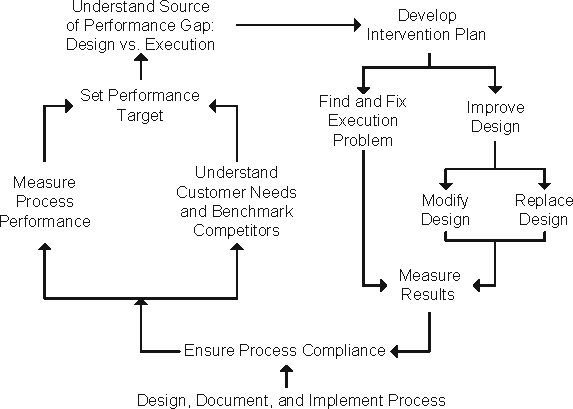
\includegraphics[width=0.8\textwidth]{Images/process_management_cycle.pdf}
\caption[Essentieller Zyklus der Geschäftsprozessmodellierung]{Essentieller Zyklus der Geschäftsprozessmodellierung \citep[S. 5]{Brocke2014}}
\label{process_management_cycle}
\end{figure}
\subsection{Business Process Mapping und Business Process Modeling}\label{subsec:BPMappingModeling}
Die Ermittlung und Visualisierung von Geschäftsprozessen stellt eine Teildisziplin im Management von Geschäftsprozessen dar. Gleichzeitig ist sie der Schlüssel zur Anpassung der Geschäftsprozesse, da ein genaues Verständnis der Abläufe für die Anpassung und Verbesserung unerlässlich sind \cite[vgl.][S. 6]{Jacka2009}. Mit dieser Problemstellung befassen sich sowohl Business Process Mapping als auch Business Process Modeling. Der Unterschied zwischen beiden besteht im wesentlichen in der Zielstellung und der damit verbundenen Abstraktionsebene \cite[vgl.][]{Smartdraw}. Process Mapping zielt im Kern auf die Dokumentation eines bestehenden Prozesses ab, weswegen das Unternehmen auf makroskopischer Sicht analysiert wird. Dabei werden die wesentlichen Funktionen und Rollen bei der Transformation des Inputs zum Output betrachtet. Process Modeling hingegen versucht bestehende Prozesse im Detail zu analysieren, um Engpässe aufzudecken und die Effizienz durch Anpassungen zu steigern \cite[vgl.][]{Appian}. Aus diesem Grund sind die dabei entstehenden Modelle detaillierter. Beide Disziplinen verwenden dabei im Idealfall standardisierte Beschreibungssprachen, wobei sich aus der höheren Detailtiefe beim Process Modeling eine höhere notwendige Komplexität der Beschreibungssprache ergibt. Aufgrund der vielen inhaltlichen und methodischen Überschneidungen der beiden Disziplinen kommt es leider häufig zu Verwechslungen beziehungsweise zur synonymen Verwendung beider Bezeichnungen \cite[vgl.][]{Smartdraw}.

Zu den allgemeinen Vorteilen von Process Mapping zählen die bessere Dokumentation der Prozesse, die Möglichkeit den Prozess grafisch zu visualisieren sowie die komplette Sicht auf die vielen verschiedenen Aspekte eines Prozesses \cite[vgl.][S. 8]{Jacka2009}. Neben diesen offensichtlichen Vorteilen gibt es allerdings noch zahlreiche weitere positive Aspekte, deren Wirkungsweise sich erst auf den zweiten Blick erschließt. Beispielsweise erhöht sich die Transparenz der Unternehmensprozesse, wodurch jeder Prozessteilnehmer seine Rolle im kompletten Kontext besser einschätzen kann. Dadurch wird die Wirkung der eigenen Tätigkeiten wesentlich klarer, was das Stolzgefühl der Mitarbeiter stärkt und so zu einer allgemeinen Steigerung der Mitarbeiterzufriedenheit führt. Zudem kann jeder Teilnehmer wesentlich mehr zur stetigen Verbesserung der Prozesse beitragen, da jedem ein holisitischer Blick auf den Prozess gewährt wird. Ein weiterer positiver Nebeneffekt ist die sich zwangsläufig ergebende Kundenorientierung, da für ein sinnvolles analysieren der Prozesse der Blick auf den für den Kunden generierten Output notwendig ist \cite[vgl.][S. 8-11]{Jacka2009}.

Prinzipiell besitzt auch Process Modeling ähnliche Vorteile, wie die bereits für Process Mapping aufgeführten. Aus der Abstraktionsebene und dem sich daraus ergebenden Detaillierungsgrad ergeben sich jedoch weitere Vorteile. Hierbei ist beispielsweise zu erwähnen, dass die Einarbeitung neuer Mitarbeiter durch die entsprechende Prozessdokumentation leichter fällt und dadurch Zeit eingespart werden kann. Durch die Modellierung der Prozesse entsteht sozusagen ein "`Prozesskatalog"' der auch als zentrales Nachschlagewerk fungieren kann. Zudem erlaubt der Detaillierungsgrad der Prozessmodelle, dass Teilaufgaben automatisiert werden können, was einen großen Vorteil darstellt. Dazu wird eine sogenannten Process Engine verwendet, die für den Nutzer beziehungsweise den Mitarbeiter als Schnittstelle zu genormten Prozessen fungiert. Standardaufgaben, wie beispielsweise das Weiterleiten eines Beurteilungsbogens nach der Prüfung, können dann automatisch durch die \ac{IT} ausgeführt werden \citep[vgl.][S. 2-8]{Freund2014}.

\subsection{BPMN 2.0}\label{subsec:BPMN}
Wie in den vorigen Abschnitten erwähnt wurde, nimmt die Visualisierung von Geschäftsprozessen einen wichtigen Standpunkt ein. \ac{BPMN} wird neben anderen Modellierungssprachen wie YAWL, EPK, Petrinetze, UML speziell im Rahmen des Business Process Modeling verwendet \cite[vgl.][S. 9]{Kossak2014}. Mit der ersten veröffentlichen Version im Jahre 2004 durch die \ac{BPMI} gilt BPMN als einer der jüngeren Vertreter der Prozessmodellierungssprachen. 2005 wurde die \ac{BPMI} durch die \ac{OMG} übernommen, die sich in der IT-Welt bereits durch die Entwicklung und Wartung von UML einen Namen gemacht hat. In der Folge wurde der Standard weiterentwickelt, bis er 2011 in der aktuellsten Version 2.0 verabschiedet werden konnte \citep[vgl.][S. 8f.]{Freund2014}. Die Aufnahme in den ISO 19510:2013 Standard und nicht zuletzt die Pflege der Sprache durch die OMG haben den Stellenwert der BPMN in der Vergangenheit stärken können und ihren Einfluss vergrößert \cite[vgl.][S.10f.]{Kossak2014}. Zudem scheint speziell im Vergleich mit anderen Modellierungssprachen der Fokus und der Blickwinkel der Sprache bei der Modellierung industrieller Prozesse am besten den Forderungen der Unternehmen zu entsprechen \cite[vgl.][S.16]{Kossak2014}. Der Vorteil liegt hier darin, dass BPMN eine angenehme Lösung für den Zielkonflikt zwischen Verständlichkeit für alle Betrachter und notwendiger Komplexität zur Modellierung detaillierter Zusammenhänge darstellt \citep[vgl.][S. 11f.]{Freund2014}.

Obwohl auch BPMN nicht fehlerfrei ist und der Standard teilweise Definitionslücken und Inkonsistenzen aufweist sowie fehlende Standardisierung bei den erstellten Modellen zu Inkompatibilitäten zwischen den verschiedenen Tools führt, erscheint es durchaus wahrscheinlich, dass sich diese Modellierungssprache in naher Zukunft als de facto Standard etablieren wird \cite[vgl.][S.161]{Kossak2014}.

Zur Unterstützung beim Verständnis der folgenden Kapitel folgt ein kurzer Überblick zu den Modellierungselementen und Konzepten von \ac{BPMN} 2.0. Der Standard, der auch die Grundlage für die folgenden Ausführungen bildet, wird von der \ac{OMG} in \citep{OMG2011} definiert.

\subsubsection{Elemente der Modellierung}\label{subsubsec:BPMNElemente}

Mit dem Fokus auf Einfachheit und Nachvollziehbarkeit werden die Elemente in \ac{BPMN} in die folgenden fünf Gruppen unterteilt:
\begin{enumerate}
\item Flussobjekte
\item Verbindende Objekte
\item Artefakte
\item Teilnehmer (Pools und Lanes)
\item Daten
\end{enumerate}
Ihre grafische Darstellung ist in Abbildung \ref{bpmn_basic_elements} zu sehen. Über eine Art visueller Notation in Gruppen ist es möglich, die Klasse oder Funktionalität von Elementen aufgrund ihrer Form einzuschätzen. Beispielsweise werden Ereignisse immer in Form eines Kreises dargestellt, wobei auch die Größendimension der verschiedenen Objekte gleich ist.
\begin{figure}[ht]
\centering
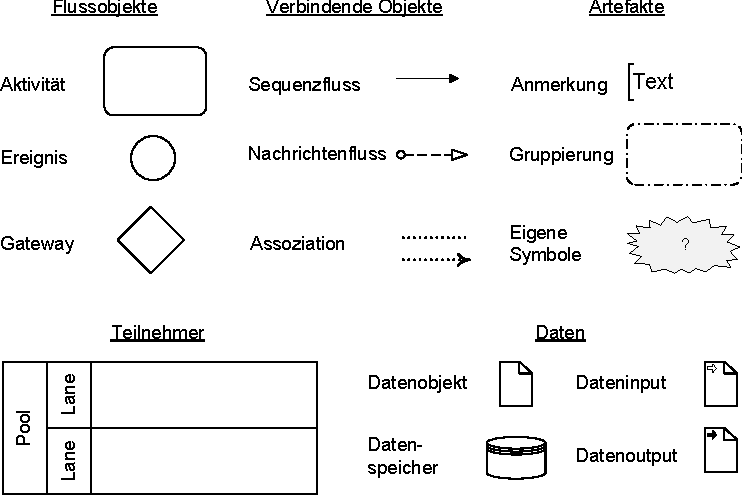
\includegraphics[width=1\textwidth]{Images/bpmn_basic_elements}
\caption[Die Basiselemente der BPMN 2.0]{Die Basiselemente der BPMN 2.0 \citep[S. 23]{Freund2014}}
\label{bpmn_basic_elements}
\end{figure}

Flussobjekte stellen die Kernelemente der Visualisierung dar und beschreiben das Verhalten des Geschäftsprozesses. Dazu unterteilen sich Flussobjekte in Aktivitäten, Ereignisse und Gateways \citep[vgl.][S. 29]{Laliwala2014}. Aktivitäten und Ereignisse erklären sich über ihren Namen sehr gut von allein und stehen somit stellvertretend für durchgeführte Aktionen (Aktivitäten) oder eintretende Ereignisse oder "`Dinge", 'die passieren können. Gateways wiederum stellen bedingte Verzweigungen dar und sind somit essentiell für komplexere Abläufe \citep[vgl.][S. 23]{Freund2014}.

Über den Sequenzfluss wird festgelegt, welche Elemente miteinander verbunden werden und in welcher Reihenfolge (angezeigt durch die Pfeilrichtung) die Elemente abgearbeitet werden. Diese Form des Prozessflusses findet allerdings nur innerhalb eines Pools oder einer Lane statt, weswegen für poolübergreifende Interaktionen Nachrichtenflüsse notwendig sind. Generell werden mit Pools und Lanes verschiedene Rollen, Personen oder andere Entitäten unterschieden und einzelne Elemente durch ihre Position innerhalb einer Lane oder eines Pools den entsprechenden Entitäten zugewiesen. Artefakte sollen zusätzliche Hinweise zum Prozess geben, ohne seine konkrete Ausführung zu verändern. Zur Verbindung von Artefakten mit anderen Objekten werden Assoziationen verwendet. Datenobjekte lassen darauf schließen, welche Daten im Laufe eines Prozesses entstehen oder verwendet werden und lassen sich ebenfalls über Assoziation mit Aktivitäten verknüpfen \citep[vgl.][S. 23f.]{Freund2014}. 
\subsubsection{Diagramm, Prozessmodell und -instanz}\label{subsubsec:BPMNModellInstanz}
Für das eindeutige Verständnis sollten die beiden Begriffe Prozessmodell und Prozessinstanz und der Unterschied zwischen beidem bekannt sein. Ein Prozessmodell beschreibt die modellierte Abbildung der Realität, also eines Prozesses, wovon ein oder mehrere in einem Diagramm enthalten sein können. Von einer Prozessinstanz wird gesprochen, wenn es um eine konkrete Ausführung eines Modells geht. Somit können mehrere Prozessinstanzen vom gleichen Prozessmodell aktiv sein. Man könnte dies auch als einen "`Vorgang"' beschreiben \citep[vgl.][S. 25f.]{Freund2014}.
\subsubsection{Token}\label{subsubsec:BPMNToken}
Das Token ist ein theoretisches Konzept, was bei der Analyse und dem Verständnis eines Prozessmodells hilft. Dabei stellt das Token ein Objekt dar, das in einem Start Event erstellt wird,  das Modell entlang der Fluss- und Verbindungselemente durchläuft und in der Regel durch ein End Event konsumiert wird. Solange ein Token im Prozessmodell "`unterwegs"' ist, bleibt die Instanz aktiv \citep[vgl.][S. 27]{OMG2011}. Gateways besitzen in diesem Zusammenhang eine besondere Bedeutung, da sie abhängig von ihrer Funktion Token vervielfachen oder verringern (konsumieren) können. Wie das Konzept des Tokens bei der Analyse verwendet wird, kann im folgenden Abschnitt bei der Erklärung eines konkreten Beispiels entnommen werden.
\subsubsection{Beispiel}\label{subsubsec:BPMNBeispiel}
Mit Hilfe eines Beispiels soll die Notation der BPMN und das Token-Konzept näher erläutert werden. Aus diesem Grund wurde ein Beispiel aus \citep{OMG2010} gewählt, welches allgemein leicht verständlich ist, aber trotzdem einen guten Querschnitt über die verfügbaren Modellierungselemente der BPMN 2.0 darstellt. Im gewählten Beispiel, das in Abbildung \ref{bpmn_pizza_collaboration} dargestellt wird, wird der Bestell- und Liefervorgang einer Pizza modelliert.
\begin{figure}[ht]
\centering
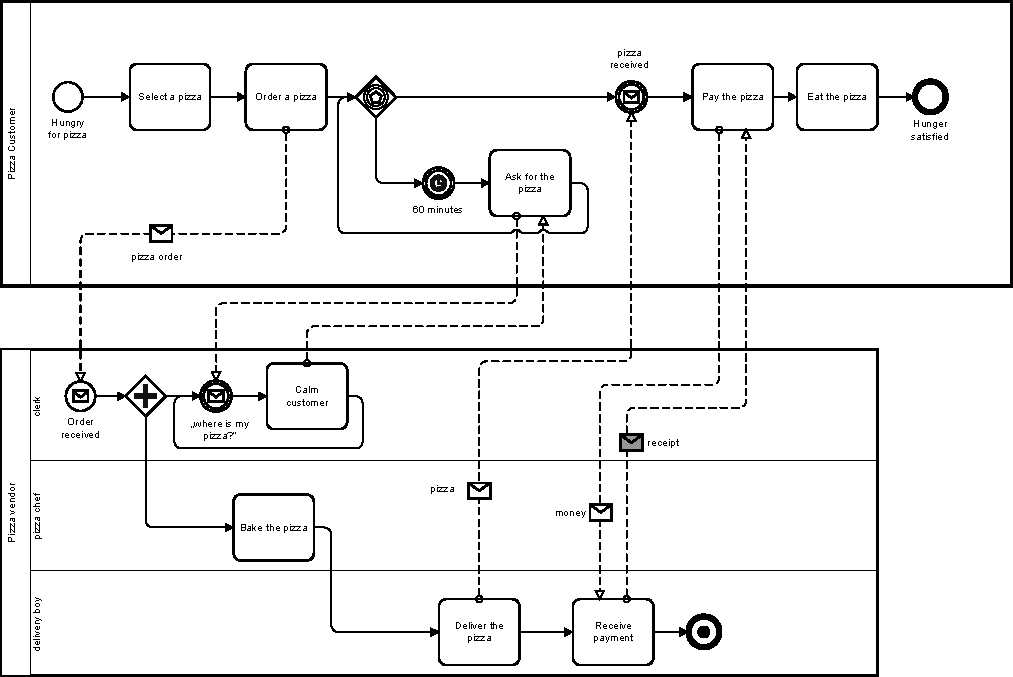
\includegraphics[width=1\textwidth]{Images/pizza_collaboration}
\caption[Bestell- und Liefervorgang einer Pizza]{Bestell- und Liefervorgang einer Pizza \citep[S. 4]{OMG2010}}
\label{bpmn_pizza_collaboration}
\end{figure}

Als erstes ist zu erkennen, dass der gesamte Prozess durch 2 Pools umgesetzt wird. Ein Pool symbolisiert in der BPMN immer eine übergeordnete Instanz, die die darin eingebetteten Lanes steuert. Eine Lane wiederum steht für eine Rolle im Prozess, die entsprechend ihrer Rolle Aufgaben durchführt oder abarbeitet. Diese Denkweise wird von dem Ziel der Automatisierung der Prozesse getrieben, da eine zentrale steuernde Instanz im Kontext eines Prozesses durch eine Process Engine sehr leicht abgelöst werden kann \citep[vgl.][S. 96ff.]{Freund2014}.

Das Startereignis liegt beim Konsumenten der Pizza, der Hunger auf eine Pizza verspürt. An dieser Stelle wird das Token generiert, was dann zu den nächsten Prozessschritten weiterläuft. Nachdem eine passende Pizza ausgewählt wurde, wird der eigentliche Bestellvorgang ausgelöst. Dazu wird, vermutlich durch einen Anruf oder per Onlinebestellung, eine Nachricht ("`pizza order"') für die Bestellung an den Angestellten des Pizzaverkäufers abgesetzt, was durch den gestrichelten Signalfluss und den Brief angezeigt wird. Anschließend wartet der Kunde auf seine Bestellung. Durch das eventbasierte Gateway wird abhängig vom ersten eingetroffenen Ereignis entweder der Bezahlvorgang eingeleitet (bei Erhalt der Pizza) oder beim Lieferanten nachgefragt, wo die Bestellung bleibt. Das Token verweilt somit im Gateway, bis eines der beiden Ereignisse ausgelöst wird, um dann dem ersten Ereignis zu folgen (XOR-Logik). Für den Bezahlvorgang wird ebenfalls der Austausch von Nachrichten zur Übergabe des Geldes und zum Erhalt der Zahlungsbestätigung verwendet. Anschließend kann der Kunde die Pizza essen und das Token wird im Abschlussevent konsumiert.

Auf der Seite des Pizzaverkäufers signalisiert der Erhalt der Nachricht für die Bestellung den Start. An dieser Stelle wird folglich das Token generiert und läuft in das parallele Gateway. Im parallelen Gateway wird das Token vervielfältigt und es startet auf jeder aus dem Gateway laufenden Prozesslinie ein Token. Eines der Token ist für die Beantwortung der Nachfragen des Kunden zuständig und wartet auf die entsprechende Nachricht, um den Kunden anschließend zu beruhigen. Das zweite Token läuft zum Pizzachef, der die bestellt Pizza bäckt. Danach wird der Prozess beim Botenjungen fortgesetzt, der die Pizza ausliefert und die Bezahlung erhält. Am Ende des Prozesses des Pizzaverkäufers gibt es mit dem Terminierungsereignis noch eine Besonderheit. In diesem Fall reicht ein normales Abschlussereignis nicht aus, da der Prozess ansonsten nie enden würde. Der Grund liegt in dem Zweig, der sich um die Kundennachfragen kümmert. Das Token, das aus dem parallelen Gateway in diese Schleife gestartet ist, kann niemals konsumiert werden, da es selbst nach Auslieferung der Pizza noch auf Nachfragen des Kunden warten würde. Aus diesem Grund wird mit Hilfe des Terminierungsereignisses der gesamte Prozess beendet und alle noch aktiven Token sofort gelöscht.

\section{Regulatorische Anforderungen für Medizingeräte}\label{sec:RegRequ}

\subsection{Gründe und Bedeutung der Regulierung für Medizinprodukte}\label{subsec:Gruende}
\subsection{Überblick über die wichtigsten Normen}\label{subsec:UeberblickNormen}
\subsection{Auswirkungen auf die Entwicklung und den Produktlebenszyklus}\label{subsec:AuswirkungenAufEntwicklung}
\subsubsection{Requirements Engineering}
\subsubsection{Product Lifecycle Management}

\section{Qualitätsprozesse nach Markteinführung medizinischer Geräte}\label{sec:PMProzesse}
\subsection{Vigilance System}\label{subsec:Vigilance}
\subsection{Post Market Surveillance}\label{subsec:PMS}
\subsection{Post Market Clinical Follow-Ups}\label{subsec:PMCF}
\subsection{Integration in die Entwicklungsprozesse}\label{subsec:IntegrationInDevProzesse}

%===================================================================== Chapter 3
\chapter{Aufnahme des Status Quo}\label{chap:AufnahmeStatusQuo}

%===================================================================== Cahpter 4
\chapter{Anpassung des Prozesses unter Berücksichtigung der Medizinprodukteverordnung (MDR) EU 2017/745}\label{chap:AnpassungAnMDR}

%===================================================================== Chapter 5
\chapter{Integration und Umsetzung des neu modellierten Prozesses}\label{chap:Integration}

%===================================================================== Zusammenfassung
\chapter{Zusammenfassung}\label{chap:Zusammenfassung}

%===================================================================== Diskussion
\chapter{Diskussion}\label{chap:Diskussion}

%===================================================================== Vorlagen
%\chapter{}\label{chap:}
%\section{}\label{sec:}
%\subsection{}\label{subsec:}
%\subsubsection{Requirements Engineering}  -- besitzt keine Nummerierung und taucht nicht im toc auf
%\cite[S. X]{<reference>}
%\ac{<Abkürzung>}

%===================================================================== Literaturverz.
\bibliography{literatur}
\bibliographystyle{alphadin}
%\bibliographystyle{abbrv}
% Übersicht unter: https://de.wikibooks.org/wiki/LaTeX-W%C3%B6rterbuch:_bibliographystyle

%===================================================================== Anhang
\appendix
\chapter[Anhang]{}
\newpage
\section{Anhang 1}

%===================================================================== Eidessattl. Vers.
\chapter*{Eidesstattliche Versicherung} %  *-> erstellt unnummeriertes chapter
Ich versichere, dass ich die vorliegende Arbeit selbstständig verfasst, keine anderen als die angegebenen Quellen und Hilfsmittel benutzt sowie alle wörtlich oder sinngemäß übernommenen Stellen in der Arbeit gekennzeichnet habe.
\\[2cm]
\noindent\rule{0.35\textwidth}{0.3pt}\rule{0.2\textwidth}{0pt}\rule{0.45\textwidth}{0.3pt}
\\Ort, Datum\rule{0.418\textwidth}{0pt}Unterschrift
\end{document}